\section{Mixnät}
\begin{frame}
\frametitle{Innehåll}
\tableofcontents[currentsection]
\end{frame}

\begin{frame}{Mixnät - översiktligt}

\begin{itemize}
\item Digital tombola
\end{itemize}

\begin{center}
  \makebox[\textwidth]{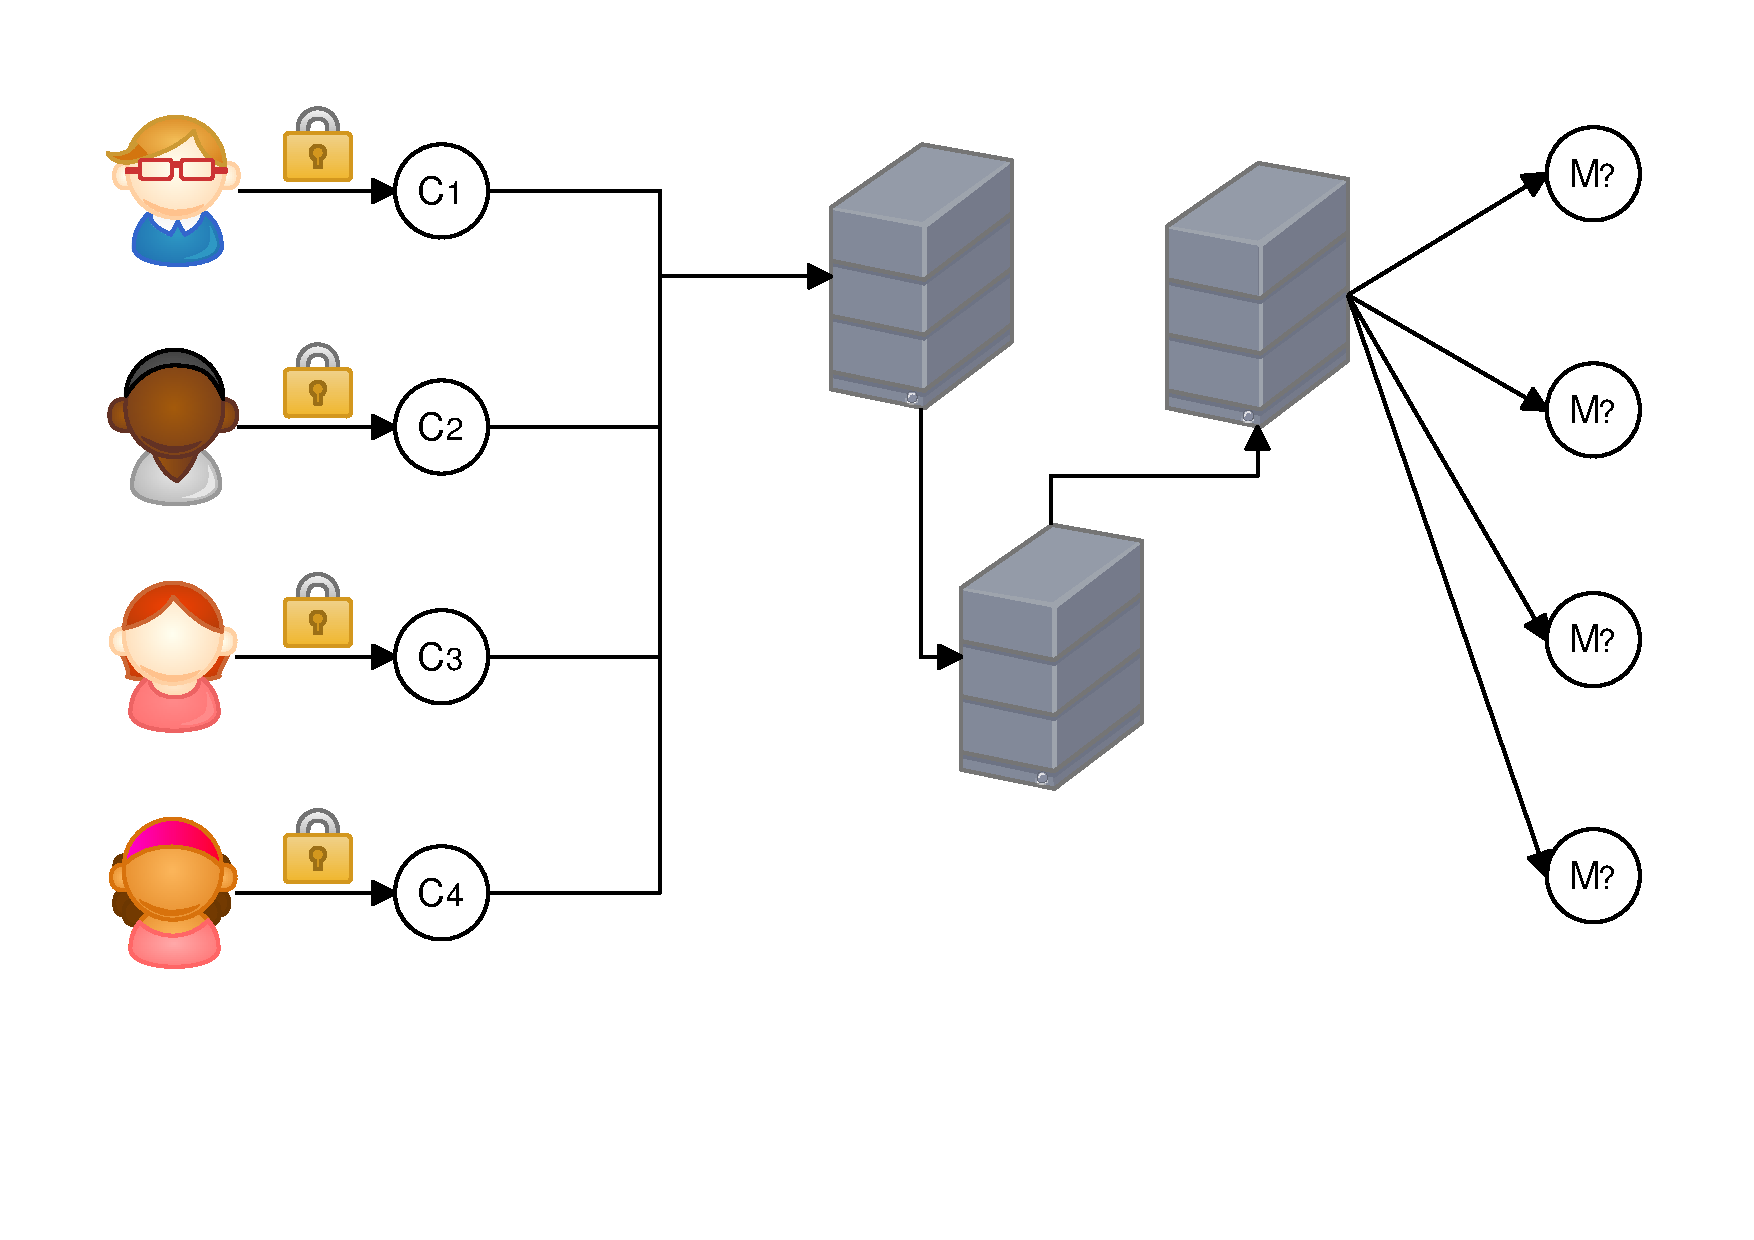
\includegraphics[height=0.9\textheight]{images/mix1.pdf}}
\end{center}

%%  Skapandet av kryptotextslistan ¨ar utanf¨or v˚art arbete. Listan g˚ar igenom noderna och krypteras om och blandas. Vi f˚ar ut en lista med r¨oster och kan inte veta vem som r¨ostat p˚a vad. F¨or att kunna g˚a igenom detaljer beh¨ovs lite krypto.

\end{frame}